% ----------------------------------------------------------------------

\chapter{\textbf{Arquitetura baseada em Micro-serviços}} % Este comando é utilizado para criar capítulos

Com a crescente demanda de recursos computacionais distribuída, o enfrentamento com problemas de gestão e custo computacional  cresceram de forma acentuada, a forma de escalar os serviços de internet, em grande parte era feita de forma vertical (Scaling up), ou seja, aumentando a quantidade de recursos da máquina, como memória ou processadores para suprir determinada demanda. Pensando em uma forma mais eficiente de disponibilizar serviços na internet, surge o padrão de arquitetura baseada em micro-serviços, onde invés de existir um único e complexo serviço, as aplicações são desenvolvidas em partes, de maneira que cada serviço funcione de forma isolada, entretanto, para o usuário final, a percepção é que a aplicação é única. 

\begin{figure}[h!]
	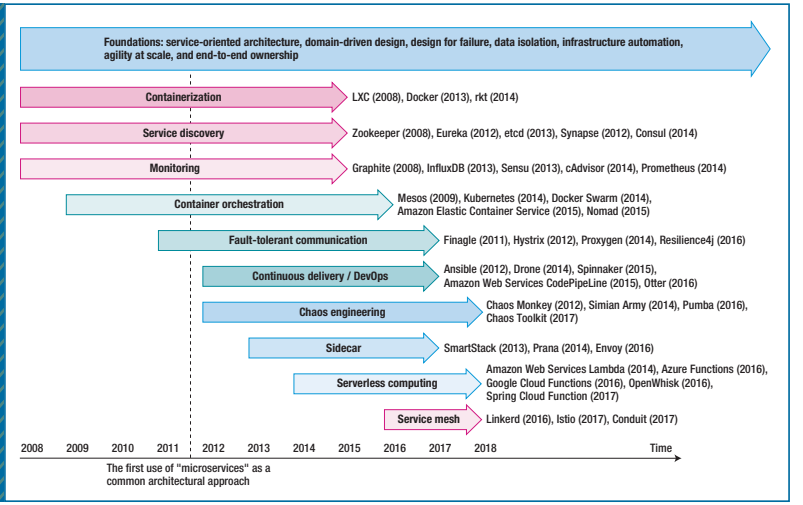
\includegraphics[width=\linewidth]{topics/timeline.png}
	\caption{Linha do tempo das tecnológica do micro-serviços, por \cite{8354433}.}
	\label{fig:timelinemicroservices}
\end{figure}


O surgimento do termo micro-serviços é recente, segundo \cite{8354433}, o termo tem início em palestras sobre arquitetura de softwares, evoluindo até os dias atuais. A princípio, são inúmeras vantagens de utilização desse tipo de arquitetura, desde a melhor divisão de trabalho entre times, (cada equipe fica responsável por uma 'pequena' parte da aplicação), custo de infraestrutura reduzido (existe a possibilidade de escalar uma aplicação em demanda da utilização de forma mais coesa), eficiência energética e custo reduzido (poder computacional estará sendo escalado sob  demanda) e a possibilidade de escala horizontal (Scaling out, onde invés de incrementar recursos computacionais, é aumentado a quantidade de máquinas que realizam a tarefa).
